\section{Related Work}
\label{sec:related_work}


%\subsubsection{Data-driven Human Motion Synthesis}
%
%Traditional human motion synthesis frameworks often rely on concatenative approaches such as \emph{motion graph} \cite{Kovar2002_MotionGraphs}. Recently, learning-based methods with neural networks have been widely applied to this area to generate high-quality and interactive motions, using models ranging from feed-forward network \cite{holden2017phase,Starke2022_DeepPhase} to dedicated generative models~\cite{henter2020moglow, Ling2020_MotionVAE}. Dealing with the one-to-many issue where a variety of motions can correspond to the same input or control signal is often a challenge for these learning-based approaches. Previous systems often employ additional conditions, such as contacts \cite{starke2020local} or phase indices \cite{holden2017phase,Starke2022_DeepPhase}, to deal with this problem. Closer to the gesture domain is the speech-driven head motion synthesis, where conditional GANs \cite{sadoughi2018novel}, and conditional VAEs \cite{greenwood2017predicting} have been used.
%
%\subsubsubsection{Music-driven Dance Synthesis}
%Among the general motion synthesis tasks, music-driven dance generation addresses a similar problem to the co-speech gesture synthesis, where the complex temporal relation between two different modalities needs to be modeled accurately. Both motion graph-based methods \cite{kim2006making,chen2021choreomaster} and learning-based approaches \cite{Li_2021_aist,valle2021transflower,li2022bailando} have been adopted and successfully achieved impressive generation results. To deal with the synchronization between the dance and music, \citet{chen2021choreomaster} develop a manually labeled rhythm signature to represent beat patterns and ensures the rhythm signatures of the generated dance match the music. \citet{aristidou2021rhythm} segment the dance into blocks at music onsets, convert each block into a motion motif \cite{aristidou2018deep} that defines a specific cluster of motions, and use the motion motif to guide the synthesis of dance at the block level. \citet{li2022bailando} employ a reinforcement learning scheme to improve the rhythmic performance of the generator using a reward function encouraging beat alignment. Our rhythm-based segmentation and canonicalization framework is partially inspired by \cite{aristidou2021rhythm}. Similar to \cite{aristidou2021rhythm}, we also segment the gestures into clips at audio beats but learn a high-level representation for each clip via the vector quantization scheme \cite{oord2017neural} instead of the K-means clustering. Moreover, our framework generates gestures in blocks of motion and denormalizes the generated motion blocks to match the rhythm of the speech. In contrast, \citet{aristidou2021rhythm} synthesize dance sequences in frames conditioned on the corresponding motion motifs.
%
%\subsubsection{Co-speech Gesture Synthesis}
%The most primitive approach used to generate human non-verbal behaviors is to animate an artificial agent using the retargeted motion capture data. This kind of approach is widely used in commercial systems (e.g., films and games) because of its high-quality motion performance. However, it is not suitable for creating interactive content that cannot be prepared beforehand. Generating co-speech gestures according to an arbitrary input has been a long-standing research topic. Previous studies can be roughly categorized into two groups, i.e., rule-based and data-driven methods.
%
%\subsubsubsection{Rule-based Method}
%The idea of the rule-based approach is to collect a set of gesture units and design specific rules that map a speech to a sequence of gesture units \cite{Kipp2004_Gesture, huang2012robot, softbank2018naoqi, cassell2004beat}. \citet{wagner2014gesture} have an excellent review of these methods. The results of the rule-based methods are generally highly explainable and controllable. However, the gesture units and rules typically have to be created manually, which can be costly and inefficient for complex systems.
%
%\subsubsubsection{Data-driven Method}
%Early research in data-driven method learns the rules embedded in data and combines them with predefined animation units to generate new gestures. For example, \citet{kopp2006towards, levine2010gesture} use probabilistic models to build correspondence between speech and gestures. \citet{Neff2008Gesture} build a statistical model to learn the personal style of each speaker. The model is combined with the input text tagged with the theme, utterance focus, and rheme to generate gesture scripts, which are then mapped to a sequence of gestures selected from an animation lexicon. \citet{chiu2015predicting} train a neural classification model to select a proper gesture unit based on the speech input. More recent research has started to take advantage of deep learning and trains  end-to-end models using raw gesture data directly, which frees the manual efforts of designing the gesture lexicon and mapping rules. Gestures can be synthesized using deterministic models such as multilayer perceptron (MLP) \cite{kucherenko2020gesticulator}, recurrent neural networks \cite{hasegawa2018evaluation, yoon2019robots, yoon2020speech, bhattacharya2021speech2affectivegestures, liu2022learning}, convolutional networks \cite{habibie2021learning}, and transformers \cite{9417647}, or by learning generative models such as normalizing flow \cite{alexanderson2020style}, VAEs \cite{li2021audio2gestures, xu2022freeform}, and learnable noise codes \cite{qian2021speech}. Our method is also a data-driven framework. We learn the motion generator and the mapping between the speech and gestures from data using a combined network structure of the vector quantized variational autoencoder (VQ-VAE)~\cite{oord2017neural} and LSTM. To capture the rhythmic and semantic correspondences between the speech and gestures, we propose a multi-stage architecture that explicitly models the rhythm and semantics in different stages. An earlier system proposed by \citet{kucherenko2021speech2properties2gestures} shares a similar high-level architectural design to our framework. However, there are two key differences: (a) our method is essentially an unsupervised learning approach, which learns the gesture lexeme, style code, and the generator directly from the data without detailed annotations; and (b) our system employs an explicit beat-based segmentation scheme which is shown to be effective in ensuring temporal coherence between the speech and the gesture.
%
%\subsubsection{Multi-Modal Data Processing}
%Co-speech gesture generation is a cross-modal process involving audio, text, motion, and other information related to the speaker and the content of the speech. The representation and alignment of each modality are essential for high-quality results~\cite{8269806}. Mel-spectrogram and MFCC acoustic features are commonly used as audio features \cite{alexanderson2020style, qian2021speech, kucherenko2020gesticulator}, typically resampled into the same framerate of the motion. For the text features, pre-trained language models like BERT \cite{devlin2019bert,kucherenko2020gesticulator} and FastText~\cite{bojanowski2017enriching,yoon2020speech} have been used to encode text transcripts into frame-wise latent codes, where paddings, fillers, or empty words are inserted into a sentence to make the world sequence the same length as the motion \cite{kucherenko2020gesticulator, yoon2020speech}. Speaker's style and emotions can also be encoded by learnable latent codes \cite{bhattacharya2021speech2affectivegestures,yoon2020speech} and are resampled or padded to match the length of the speech. In this work, we employ a pre-trained speech model to extract audio features and fine-tune it using a contrastive learning strategy. We also utilize a BERT-based model to vectorize the text. These multi-modal data are then aligned explicitly using the standard approaches discussed above. Notably, a concurrent study \cite{liu2022learning} also extracts audio features using contrastive learning. Their framework considers the learning of the audio features as a part of the training of the gesture generator. Instead, our framework trains the audio encoder in a separate pre-training stage using only the audio data.
 
%\subsubsection{Evaluation of Motion Synthesis Models}
%Evaluating the generated co-speech gestures is often difficult because the motion quality is a very subjective concept. Previous works have proposed several evaluation criteria. Wolfert et al.~\shortcite{wolfert2022evaluation} have made a comprehensive review of them. User studies are widely adopted to evaluate different aspects of motion quality, such as human-likeliness and speech-gesture matching \cite{alexanderson2020style, yoon2020speech, kucherenko2020gesticulator}, but can be expensive and hard to exclude uncontrolled factors. The absolute difference of joint positions or other motion features, such as velocity and acceleration between a reconstructed motion and the ground truth, is used by several works as an objective metric \cite{ginosar2019learning, joo2019towards, kucherenko2019analyzing}. However, this metric is not suitable for evaluating motions that are natural but not the same as the reference. Fr{\'e}chet Inception Distance (FID) \cite{heusel2017gans} is a widely used criterion in image generation tasks that measures the difference between the distributions of the dataset and generated samples in the latent space. It successfully reflects the perceptual quality of generated samples. Similarly, \citet{yoon2020speech} and \citet{qian2021speech} propose Fr{\'e}chet Gesture Distance (FGD) and Fr{\'e}chet Template Distance (FTD) metrics, respectively. These metrics measure the perceptual quality of generated gestures. In this paper, we compare our framework with several baseline methods using both user studies and objective metrics like FGD. We further propose a simple but effective rhythmic metric to measure the percentage of matched beats by dynamically adjusting the matching threshold, which provides a more informative picture of the rhythm performance.

%\begin{figure*}[h]
%    \centering
%    \includegraphics[width=0.8\textwidth]{images/OHGesture.png}
%    \caption{
%    Our system is composed of DeepGesture
%    }
%    \Description{}
%    \label{fig:system_overview}
%\end{figure*}

\begin{figure*}[H]
	\centering
	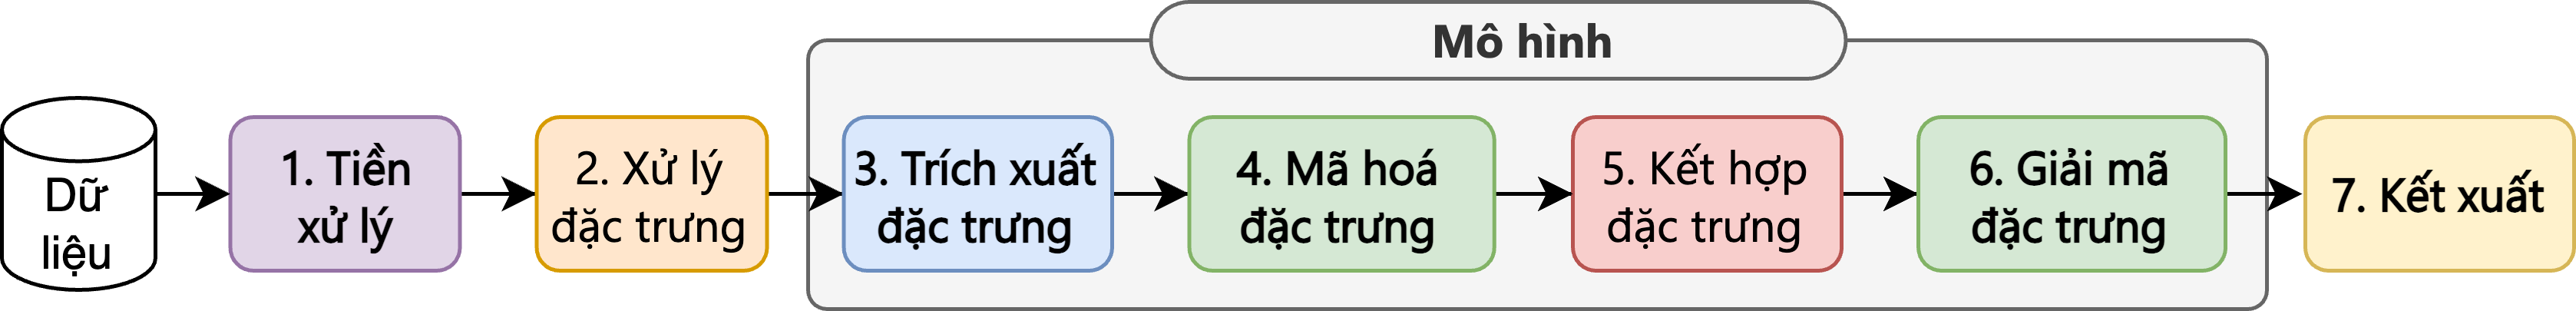
\includegraphics[width=0.8\textwidth]{images/CommonStage.png}
	\caption{Common stages in gesture generation models.}
	\Description{}
	\label{fig:CommonStage}
\end{figure*}

The gesture generation problem, like other machine learning tasks, has been studied and developed alongside both traditional and modern machine learning methods. These include rule-based and data-driven approaches. This thesis first presents the characteristics of gestures \autoref{sec:relationspeechandgesture}, serving as the foundation for learning the relationship between gestures, text, and speech. In section \autoref{sec:commonstage}, the thesis introduces the common stages across different gesture generation methods.


\subsection{Gesture Characteristics}
\label{sec:relationspeechandgesture}

According to linguistics, gestures can be categorized into six main groups: adaptors, emblems, deictics, iconics, metaphorics, and beats \cite{ekman1969repertoire}, \cite{sebeok2011advances}. Among them, beat gestures do not carry direct semantic meaning but play an important role in synchronizing rhythm between speech and gesture \cite{kipp2005gesture}, \cite{sebeok2011advances}. However, the rhythm between speech and beat gestures is not fully synchronized, making the temporal alignment between them complex to model \cite{mcclave1994gestural}, \cite{bhattacharya2021speech2affectivegestures}, \cite{kucherenko2020gesticulator}, \cite{yoon2020speech}.

Gestures interact with various levels of information in speech \cite{sebeok2011advances}. For instance, emblematic gestures like a thumbs-up are usually linked to high-level semantic content (e.g., “good” or “excellent”), while beat gestures often accompany low-level prosodic features such as emphasis. Previous studies typically extract features from the final layer of the speech encoder to synthesize gestures \cite{alexanderson2020style}, \cite{bhattacharya2021speech2affectivegestures}, \cite{kucherenko2021large}, \cite{qian2021speech}, \cite{yoon2022genea}. However, this approach may blend information from different levels, making it hard to disentangle rhythm and semantics.

As shown in linguistic studies \cite{kipp2005gesture}, \cite{neff2008gesture}, \cite{webb1997linguistic}, gestures in daily communication can be decomposed into a limited number of semantic units with various motion variations. Based on this assumption, speech features are divided into two types: high-level features representing semantic units and low-level features capturing motion variations. Their relationships are learned across different layers of the speech encoder. Experiments demonstrate that this mechanism can effectively disentangle features at different levels and generate gestures that are both semantically and stylistically appropriate.

\subsection{Overview of Gesture Generation Methods}
\label{sec:relatedwork}

\subsubsection{Rule-Based Methods}


\textbf{General Principle}: These methods rely on clearly defined rules, which are manually crafted to determine how the system processes inputs to produce outputs.

\textbf{Methods}: Representative rule-based methods include the \textit{Robot behavior toolkit} \cite{huang2012robot} and \textit{Animated conversation} \cite{cassell1994animated}. These approaches typically map speech to gesture units using handcrafted rules. Rule-based systems allow for straightforward control over model outputs and provide good interpretability.  
However, the cost of manually designing these rules is prohibitive for complex applications requiring the processing of large-scale data.

\subsubsection{Statistical Methods}


\textbf{General Principle}: These methods rely on data analysis, learning patterns from datasets, and using probabilistic models or mathematical functions for prediction. The approach involves optimizing model parameters to fit the data.


\textbf{Methods}: Like rule-based methods, data-driven methods also map speech features to corresponding gestures. However, instead of manual rules, they employ automatic learning based on statistical data analysis.

Representative statistical approaches include \textit{Gesture controllers} \cite{levine2010gesture}, \textit{Statistics-based} \cite{yang2020statistics}, which use probabilistic distributions to find similarities between speech and gesture features. \textit{Gesture modeling} \cite{neff2008gesture} constructs probabilistic models to learn individual speaker styles.

\subsubsection{Deep Learning Methods}


\textbf{General Principle of Deep Learning Methods}: These methods utilize multi-layer perceptrons (MLPs) to automatically extract features from raw data and learn complex data representations through parameter optimization.

\begin{figure}[h]
	\centering
	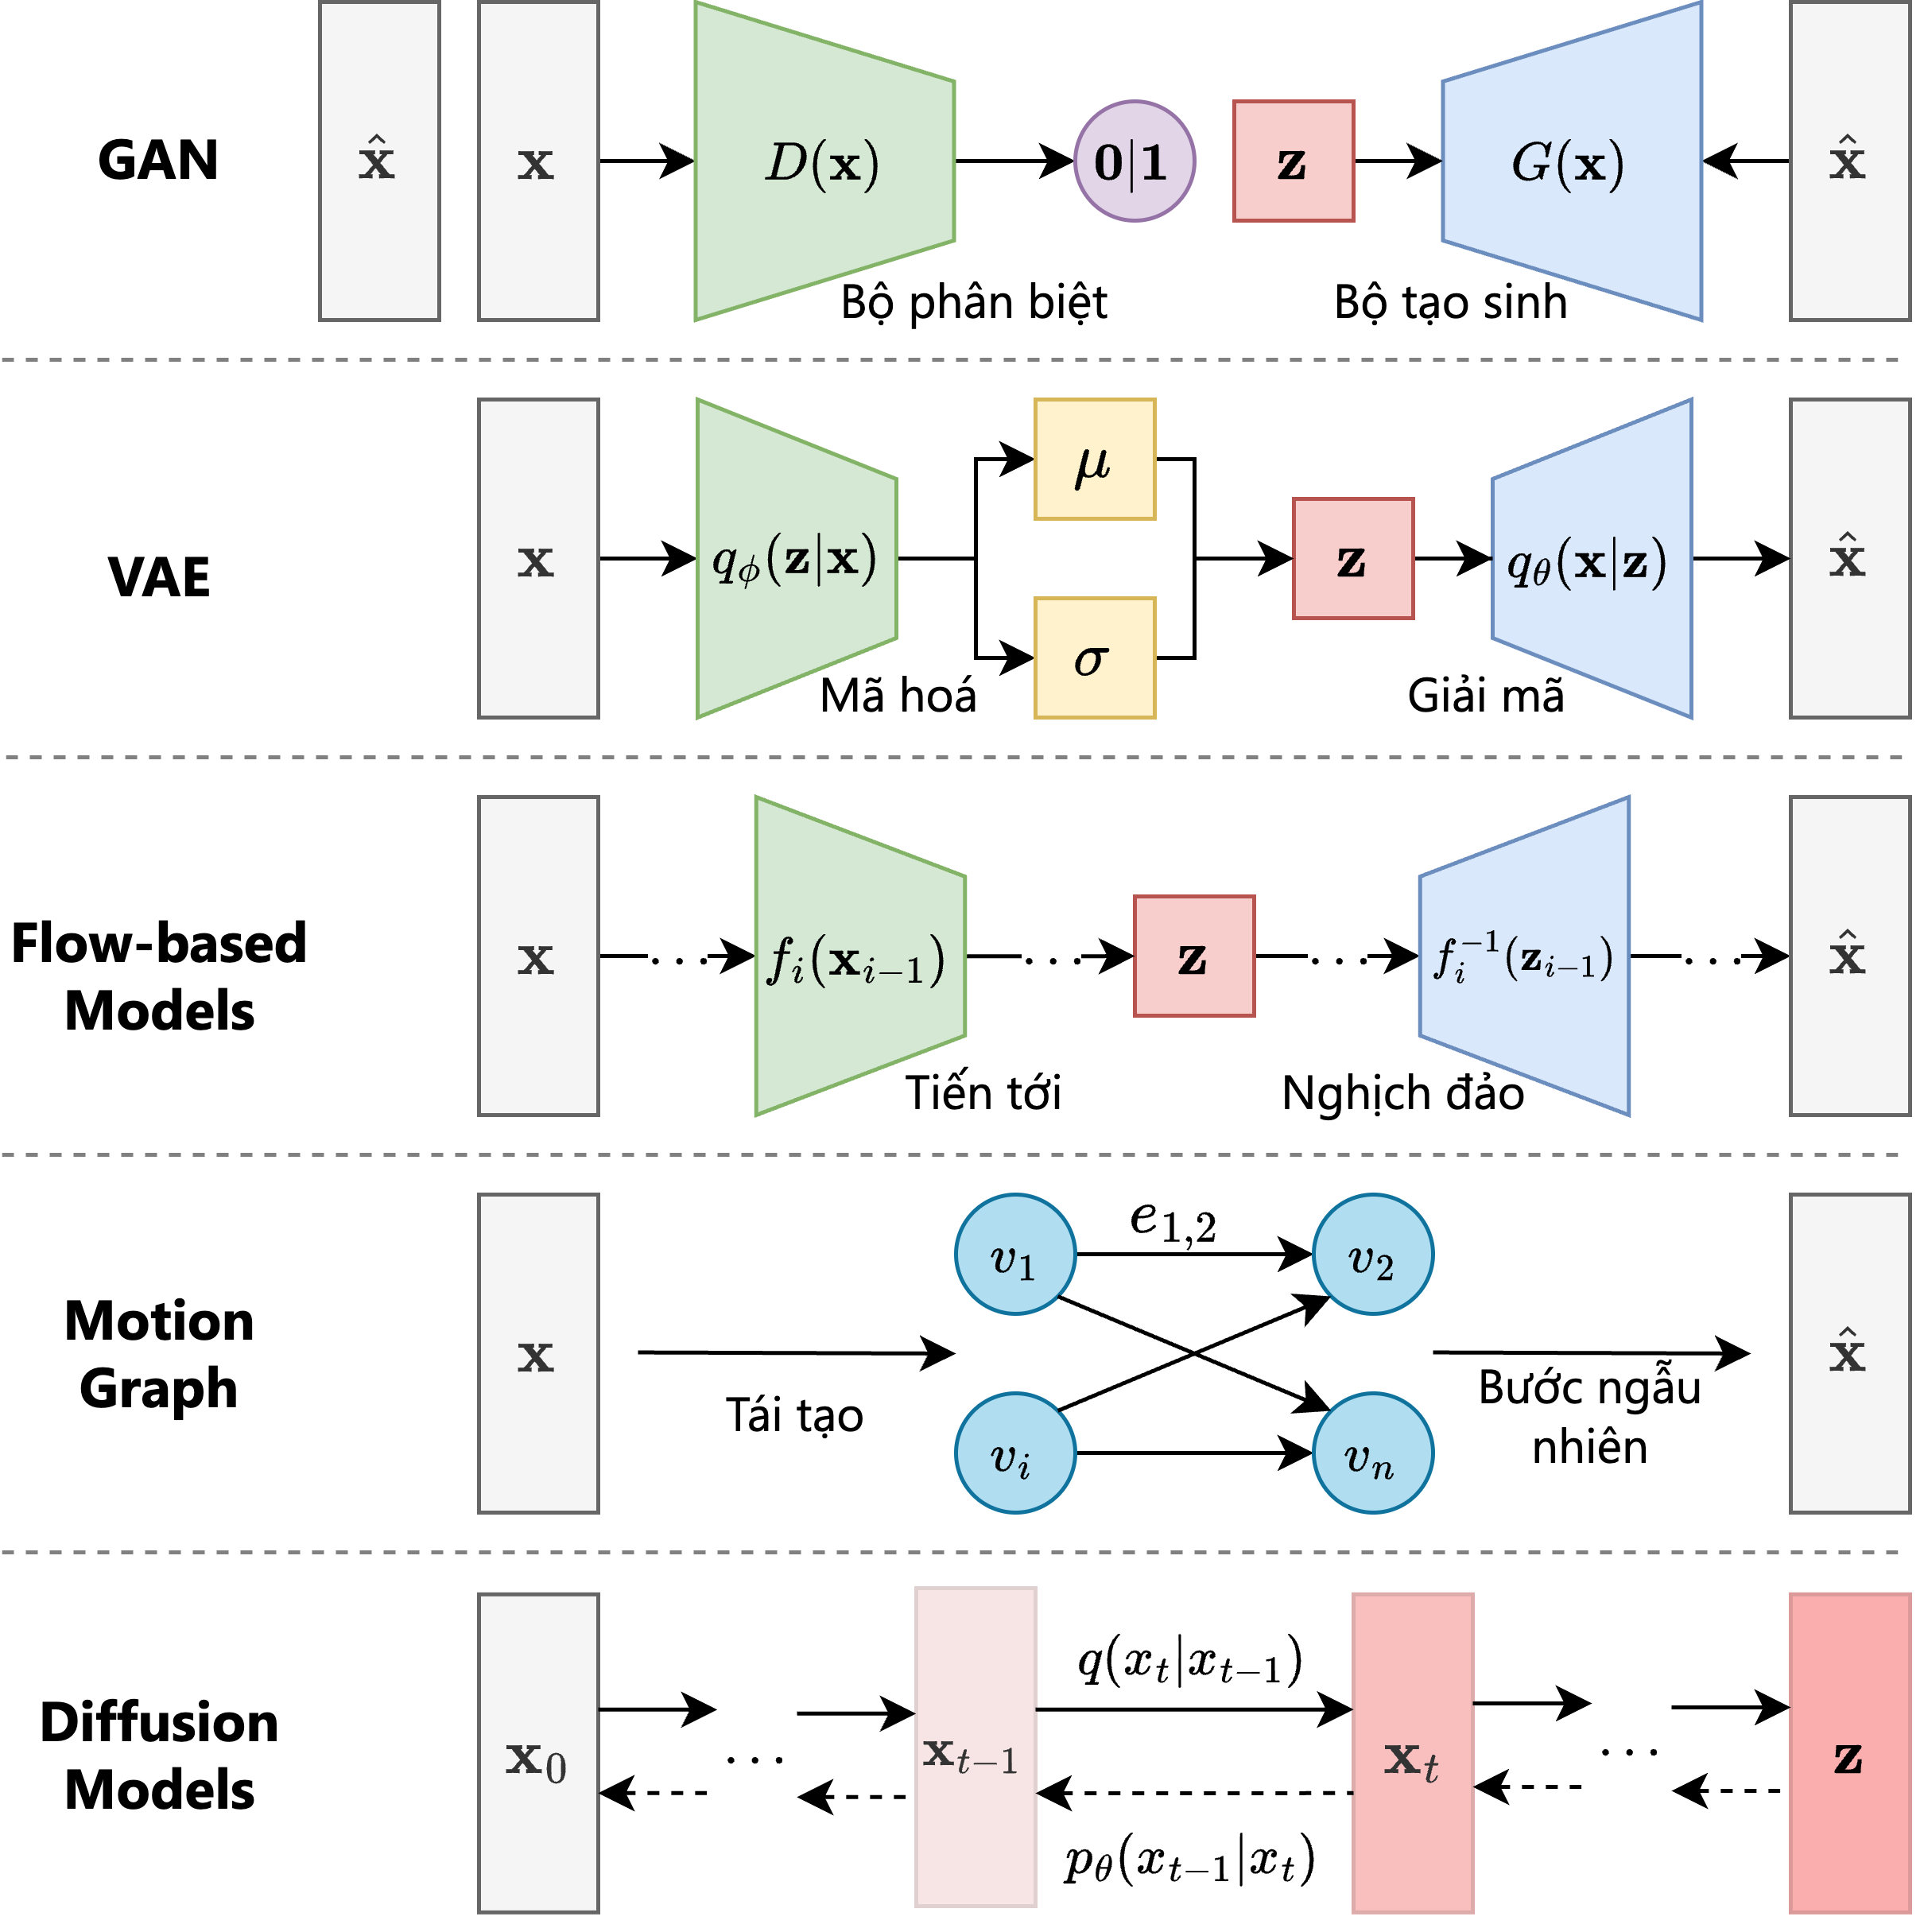
\includegraphics[width=0.8\linewidth]{images/GeneralOverview}
	\caption{Overview of different generative models.}
	\label{fig:GeneralOverview}
\end{figure}

As illustrated in \autoref{fig:GeneralOverview}, deep learning-based gesture generation methods can be divided into two main groups: likelihood-based models and implicit generative models \cite{song2021score}.


\textbf{Likelihood-Based Models}


\textbf{General Principle of Likelihood-Based Models}: These models work by maximizing the likelihood of observed data given model parameters $\theta$. The objective is to find the optimal parameters $\theta'$ by modeling the probability $p(\mathbf{x})$ of the data, where $\mathbf{x}$ represents the gesture sequence.


\textbf{Methods}: The application of deep learning to gesture generation has evolved alongside the development of deep learning models, including RNNs, LSTMs, and Transformers. Representative likelihood-based methods include:

\begin{itemize}
	\item \textit{Gesticulator} \cite{kucherenko2020gesticulator}, which uses a Multilayer Perceptron (MLP) to encode text and audio features, with BERT-derived vectors used as text features.
	
	\item \textit{HA2G} \cite{liu2022learning} builds a hierarchical Transformer-based model to learn multi-level correlations between speech and gestures, from local to global features.
	
	\item \textit{Gesture Generation from Trimodal Context} \cite{yoon2020speech} uses an RNN architecture and treats gesture generation as a translation task in natural language processing.
	
	\item \textit{DNN} \cite{chiu2015predicting} combines LSTM and GRU to build a classifier neural network that selects appropriate gesture units based on speech input.
	
	\item \textit{Cascaded Motion Network (CaMN)} \cite{liu2022beat} introduces the BEAT dataset and a waterfall-like model. Speaker information, emotion labels, text, speech, and gesture features are processed through layers to extract latent vectors. In the fusion stage, CaMN combines features sequentially: speaker and emotion features are merged first, followed by integration with latent vectors of text, speech, and gestures.
	
	\item \textbf{Motion Graph}: In \textit{Gesturemaster} \cite{zhou2022gesturemaster}, a semantic graph is constructed where words in a sentence are connected based on semantic relationships. The model then selects the most relevant nodes and edges in the graph to represent gestures.
\end{itemize}


\textbf{Implicit Generative Models}
\label{sec:ImplicitGenerativeModels}



\textbf{Principle}: Implicit generative models learn the data distribution without explicitly modeling the probability density function $p(\bx)$. Instead of directly computing $p(\bx)$, the model learns a mapping $G_{\theta}: \mathcal{Z} \to \mathcal{X}$ by matching the distributions between real and generated data $\mathbf{x} = G_\theta(\mathbf{z}), \quad \mathbf{z} \sim p_z(\mathbf{z})$. Here, $\mathcal{Z}$ denotes the input noise space, typically with a simple distribution \(p_{z}\) (e.g., Gaussian, Uniform), and \(\mathcal{X}\) is the space of real data, which in this case is gesture sequences \(\mathbf{x}\).

In gesture generation, to incorporate conditions such as speech or text labels, implicit generative models often introduce a condition $\mathbf{c}$ representing the context of the task, resulting in the conditional generation: $\mathbf{x} = G_\theta(\mathbf{z}, \mathbf{c})$. This context may include speech, text, speaker ID, style, emotion, or initial gestures.

A typical example is the generative adversarial network (GAN) and Diffusion model, where data is synthesized by transforming an initial simple distribution (e.g., Gaussian) into the target data distribution.

\textbf{Methods}: Representative implicit generative models include:

\begin{itemize}
	\item \textit{MoGlow} \cite{henter2020moglow} uses Normalizing Flows to maintain motion consistency and compatibility, while providing control via input parameters. This allows users to generate new motions or modify existing ones by adjusting control parameters.
	
	\item \textbf{GAN}: \textit{GRU-based WGAN} \cite{wu2021probabilistic} utilizes Wasserstein GAN to evaluate and improve the quality of gesture synthesis. The model focuses on optimizing the Wasserstein loss, mitigating mode collapse typically seen in traditional GANs. GRUs process speech data and convert it into usable gesture features, which are then fed into the WGAN for evaluation and refinement.
	
	\item \textbf{VAE}: \textit{FreeMo} \cite{xu2022freeform} employs a VAE to decompose gestures into pose modes and rhythmic motions. Gesture poses are randomly sampled using conditional sampling in the VAE's latent space, while rhythmic motions are generated from...
	
	\item \textbf{VQ-VAE}: \textit{Rhythmic Gesticulator} \cite{ao2022rhythmic} preprocesses speech segments based on beats, dividing speech into smaller parts and representing them as blocks with normalized dimensions. Similar to the VQ-VAE approach, normalized gesture sequences are quantized into discrete gesture lexicons. The model learns the gesture vocabulary conditioned on the previous gesture, gesture style, and speech. It then reconstructs the gesture sequence via denormalization. Unlike generative models like GANs or Diffusion, VQ-VAE focuses more on compression rather than direct generation.
	
	\item \textbf{Diffusion}: Diffusion models focus on generating new data from noisy inputs by progressively denoising toward the original data. Diffusion-based approaches will be presented in section \autoref{sec:diffusionbase}.
\end{itemize}

\subsubsection{Comparison of Gesture Generation Methods}


\begin{table*}[t]
	\small
	\centering
	\renewcommand{\arraystretch}{1.5}
	\resizebox{\textwidth}{!}{
		\begin{tabular}{|p{0.2\textwidth}|p{0.35\textwidth}|p{0.35\textwidth}|p{0.2\textwidth}|}
			\hline
			\textbf{Representative Method} & \textbf{Advantages} & \textbf{Disadvantages} & \textbf{Method Type} \\ \hline
			Robot behavior toolkit \cite{huang2012robot} & 
			- Easy to understand and implement. \newline 
			- Highly interpretable and controllable. \newline
			- Effective for simple cases or small datasets. & 
			- Does not generalize well to complex data. \newline 
			- Labor-intensive rule construction. & 
			Rule-based model \\ \hline
			MLP \cite{kucherenko2020gesticulator}, RNN \cite{bhattacharya2021speech2affectivegestures}, \cite{liu2022learning}, \cite{hasegawa2018evaluation}, \cite{yoon2020speech}, CNN \cite{habibie2021learning}, Transformer \cite{bhattacharya2021text2gestures}  & 
			- Able to estimate data probability density. \newline 
			- Scalable and learns well from large datasets. & 
			- Sensitive to noise. \newline 
			- Performs poorly on low-frequency data. \newline
			- Low diversity in generation. & 
			Likelihood-based model \\ \hline
			\textbf{DiffusionStyle-Gesture} \cite{yang2023diffusestylegesture}, MDM \cite{tevet2022human}, Motiondiffuse \cite{zhang2022motiondiffuse} &
			- Generates high-quality data. \newline 
			- Flexible and diverse outputs. \newline
			- Covers low-density regions of data space. & 
			- Requires complex configuration for optimal performance. \newline 
			- Random noise leads to different outputs each time. \newline 
			- Slow sampling process. & 
			Implicit generative model \\ \hline
		\end{tabular}
	}
	\caption{Comparison of advantages and disadvantages of different methods}
	\label{table:CompareMethod}
\end{table*}


